%% Presentación inicial del curso de Estructuras Discretas, 2017-1
%% Facultad de Ciencias, UNAM
%% Profa: Laura Freidberg Gojman
%% Ayudante: José Ricardo Rodríguez Abreu
%% Ayudante de lab: Albert Manuel Orozco Camacho

%% Author: AlOrozco53
%% Version: 0.0

%% Comienza el preámbulo de la presentación
\documentclass{beamer} %% clase de LaTeX utilizada para hacer diapositivas
\usetheme{Szeged} %% tema visual de la presentación
\usecolortheme{dolphin} %% combinación de colores para el tema visual
\usepackage[utf8]{inputenc} %% codificación para la inserción acentos y otros carácteres especiales
\usepackage[T1]{fontenc} %% codificación para la impresión de acentos y otros carácteres especiales
\usepackage{graphicx} %% paquete para el manejo de imágenes y gráficos externos
\usepackage{float} %% paquete que mejora la interfaz para el manejo de objetos como tablas y figuras
\usepackage{wrapfig} %% paquete que permite que el texto se ajuste entorno a figuras y tablas
\usepackage[normalem]{ulem} %% paquete que maneja varios tipos de subrayado

%% Los siguientes paquetes sirven para utilizar símbolos especiales (principalmente de matemáticas)
\usepackage{amsmath}
\usepackage{textcomp}
\usepackage{marvosym}
\usepackage{wasysym}
\usepackage{amssymb}

\usepackage{hyperref} %% paquete para manejo de hipervínculos
\tolerance=1000 %% manejo de saltos de línea
\usepackage[english, spanish]{babel} %% paquete que administra reglas y caracterísitcas de acuerdo a los idiomas especificados

%% Incrementa el nivel de comandos de sección que deben ser mostrados en el índice
\setcounter{tocdepth}{4}
\setcounter{secnumdepth}{4}

\graphicspath{{../img/}} %% directorio donde se encuentran las imágenes

%% Configuración del pie de página de cada diapositiva
\setbeamertemplate{footline}{
  \leavevmode%
  \hbox{%
    \begin{beamercolorbox}[wd=.4\paperwidth,ht=2.25ex,dp=1ex,center]{author in head/foot}%
      \usebeamerfont{author in head/foot}\insertshortauthor
    \end{beamercolorbox}%
    \begin{beamercolorbox}[wd=.6\paperwidth,ht=2.25ex,dp=1ex,center]{title in head/foot}%
      \usebeamerfont{title in head/foot}\insertshorttitle\hspace*{3em}
      \insertframenumber{} / \inserttotalframenumber\hspace*{1ex}
  \end{beamercolorbox}}%
  \vskip0pt%
}

%% Título
\title[Introducción \LaTeX]{Una Introducción a \LaTeX}

%% Autores
\author[Freidberg, Rodríguez, Orozco]{
  \small 
  \texttt{\href{mailto:lfreidberg@yahoo.com}{Laura Freidberg Gojman}}
  \and
  \texttt{\href{mailto:ricardo_rodab@ciencias.unam.mx}{José Ricardo Rodríguez Abreu}}
  \and
  \texttt{\href{mailto:alorozco53@ciencias.unam.mx}{Albert Manuel Orozco Camacho}}
}

%% Fecha de hoy
\date{\today}

%% Fin del preámbulo de la presentación

%% Comienza el cuerpo de la presentación
\begin{document}

%% Diapositiva inicial (título)
\begin{frame}
  \titlepage
  \centering 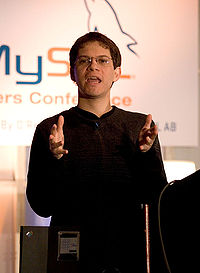
\includegraphics[scale=1]{cscientist}
\end{frame}

%% Diapositiva para el índice de la presentación
\begin{frame}
  \frametitle{Índice}
  \tableofcontents
\end{frame}

\section{Generalidades de \TeX{} y \LaTeX}

\begin{frame}
  \frametitle{¿Qué es \TeX{} y qué es \LaTeX?}
  \begin{itemize}
  \item En la década de los $70s$, \emph{Donald Knuth} desarrolló el sistema \TeX, un\
    sofisticado programa para la composición tipográfica de textos científicos y\
    técnicos.
  \item Más tarde \emph{Leslie Lamport} reunió un conjunto de \emph{macros} en un\
    \textbf{lenguaje} que permite al usuario preparar un documento con alta calidad.
  \end{itemize}
  \centering 
\includegraphics[scale=0.15]{wsucks}
\end{frame}

\begin{frame}
  \begin{itemize}
  \item \LaTeX{} permite combinar texto plano con texto en modo matemático\
    (e insertar ¡código fuente de cualquier lenguaje de programación!).
  \item Los comandos en \LaTeX{} se especifican precediéndolos de una diagonal\
    invertida ``\textbackslash''.
  \item Para insertar un comentario, se antepone a una línea un símbolo de\
    porcentaje ``$\%$''.
  \end{itemize}
\end{frame}

\section{Instalando e Iniciando}

\begin{frame}
  \frametitle{Distribuciones}
  Existen varias distribuciones de \LaTeX{} para cada sistema operativo. Las más\
  populares son:
  \begin{itemize}
  \item \href{http://miktex.org/howto/install-miktex}{\textbf{MiK\TeX}} para Windows.
  \item \href{http://milq.github.io/install-latex-ubuntu-debian/}{\textbf{\TeX Live}} para Ubuntu,\
    Debian, Mac y/o Windows.
  \item \href{https://tug.org/mactex/theinstaller.html}{\textbf{Mac\TeX}} para Mac OS X.
  \item (En los nombres de las distribuciones anterirores hay un vínculo a un manual de instalación\
    para cada una).
  \end{itemize}
\end{frame}

\subsection{Editando archivos \LaTeX}

\begin{frame}
  \frametitle{Sobre los editores de texto..}
    \begin{itemize}
    \item  Se les recomienda usar un editor de texto plano como \emph{Emacs o Vi}\
      que les permita darse cuenta de cómo trabajan las entrañas de \LaTeX
    \item Existen otros editores populares (sobre todo para Ubuntu):
      \begin{itemize}
      \item \href{http://www.xm1math.net/texmaker/}{\textbf{\TeX Maker}}
      \item \href{https://github.com/alexandervdm/gummi}{\textbf{Gummi}}
      \item \href{https://www.overleaf.com}{\textbf{Overleaf}} es un servicio en línea\
        de edición de documentos \LaTeX. Está orientado al trabajo colaborativo y\
        contiene una gran variedad de plantillas para cualquier tipo de documentos.
      \end{itemize}
    \end{itemize}
\end{frame}

\subsection{Compilación}

\begin{frame}
  \frametitle{Hay dos maneras de llevar un archivo \texttt{.tex} a un formato legible por usuarios}
  En línea de comandos, ejecutar:
  \begin{enumerate}
  \item \texttt{\$ latex archivo.tex}\\
    \texttt{\$ dviXYZ archivo.pdf}\\
    donde \texttt{XYZ} se refiere al formato de salida deseado (pdf, postscript, etcétera) 
  \item \texttt{\$ pdflatex archivo.tex}
  \end{enumerate}
\end{frame}

\section{Clases}

\begin{frame}
  \frametitle{Clases}
  \begin{flushleft}
    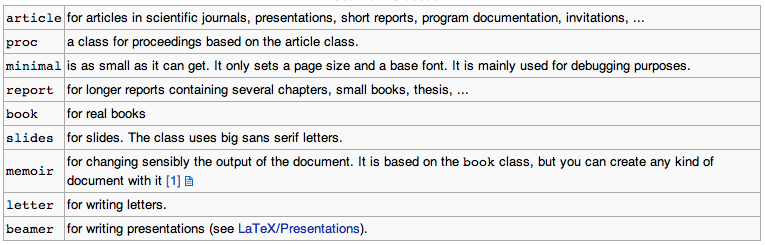
\includegraphics[scale=0.45]{classes}
  \end{flushleft}
\end{frame}

\end{document}
%% Fin del cuerpo de la presentación
